\let\textcircled=\pgftextcircled
\chapter{Combined search for the invisible decay of the Higgs boson in hadronic channels}
\label{chap:higgstoinv}

\initial{T}his is the analysis chapter on \higgstoinv.

%=======
\begin{easylist}[itemize]
\ListProperties(Style*=-- , FinalMark={)}, Margin=0.5cm)
& Discuss how the theoretical aspects from the Theory chapter translate into an experimental search.

& Discuss the necessity of including all production modes of Higgs (invisible final state, so characterise events based on initial/additional particles). Also mention how sensitive each production mode is at contributing to the branching ratio limit. Emphasise the non-VBF modes (\ggF, \ttH, \VH\ -- \WplusH, \WminusH, \ZH) in this chapter as that's what I've been working on and another student will be covering \acrshort{vbf}.

& Add a section or subsection somewhere regarding analysis tools. Perhaps add a brief description of ROOT (and how it's entrenched in HEP even though people are tending to move away from ROOT-based analysis onto more industry-standard tools), then lead into the FAST tools and using dataframes, vectorisation, etc., with only small interfaces to ROOT (for I/O) to extract data. Potentially mention how the data tiers work in CMS (RAW, DIGI, RECO, AOD, miniAOD, nanoAOD, etc.)

& Talk about what makes this analysis unique: doing a combination over all production modes from the start instead of separate analyses combined at the end. Means we can share samples, systematics, background methods and workflows, build in orthogonality between the different modes and cover as much phase space as possible (with new final states such as boosted \PZ bosons with unresolved subjets). This makes the analysis much more cohesive and consistent.

& Include object definitions, overall analysis strategy, triggers, signal production (with each non-VBF mode in detail), event selection, background estimation and results/limit (including comparisons to previous results).

& Emphasise my contributions: control region construction and studies, background estimation, and other studies I will have conducted by the time I write up.

& Current material: no public plots as of yet. Hope to finish analysis by the time I begin writing up. We are preparing a CMS internal analysis note, documenting all aspects of the analysis. I will add all relevant information there which I can subsequently use when writing this chapter.

& Since it's my thesis, I can talk about \ttH, \VH and \ggF/monojet, even though the Bristol contribution to the final, public result would only be \ttH and resolved \VH. Would need to be able to run the fit for all three modes simultaneously, ensuring we have complete (and correct) systematics for \ggF.
\end{easylist}

% Can pull from Section 37 of my lab book, and all the talks I and other people from the team have given (Presentations and talks/ folder, also Other peoples/ subdirectory). Can also pull from AN for analysis strategy



%=========================================================


\section{Analysis overview}
\label{sec:htoinv_overview}


%=========================================================


\subsection{Hadronic production modes of the Higgs boson}
\label{subsec:htoinv_production_modes}

\begin{figure}[htbp]
    \centering
    \begin{subfigure}[b]{0.45\textwidth}
        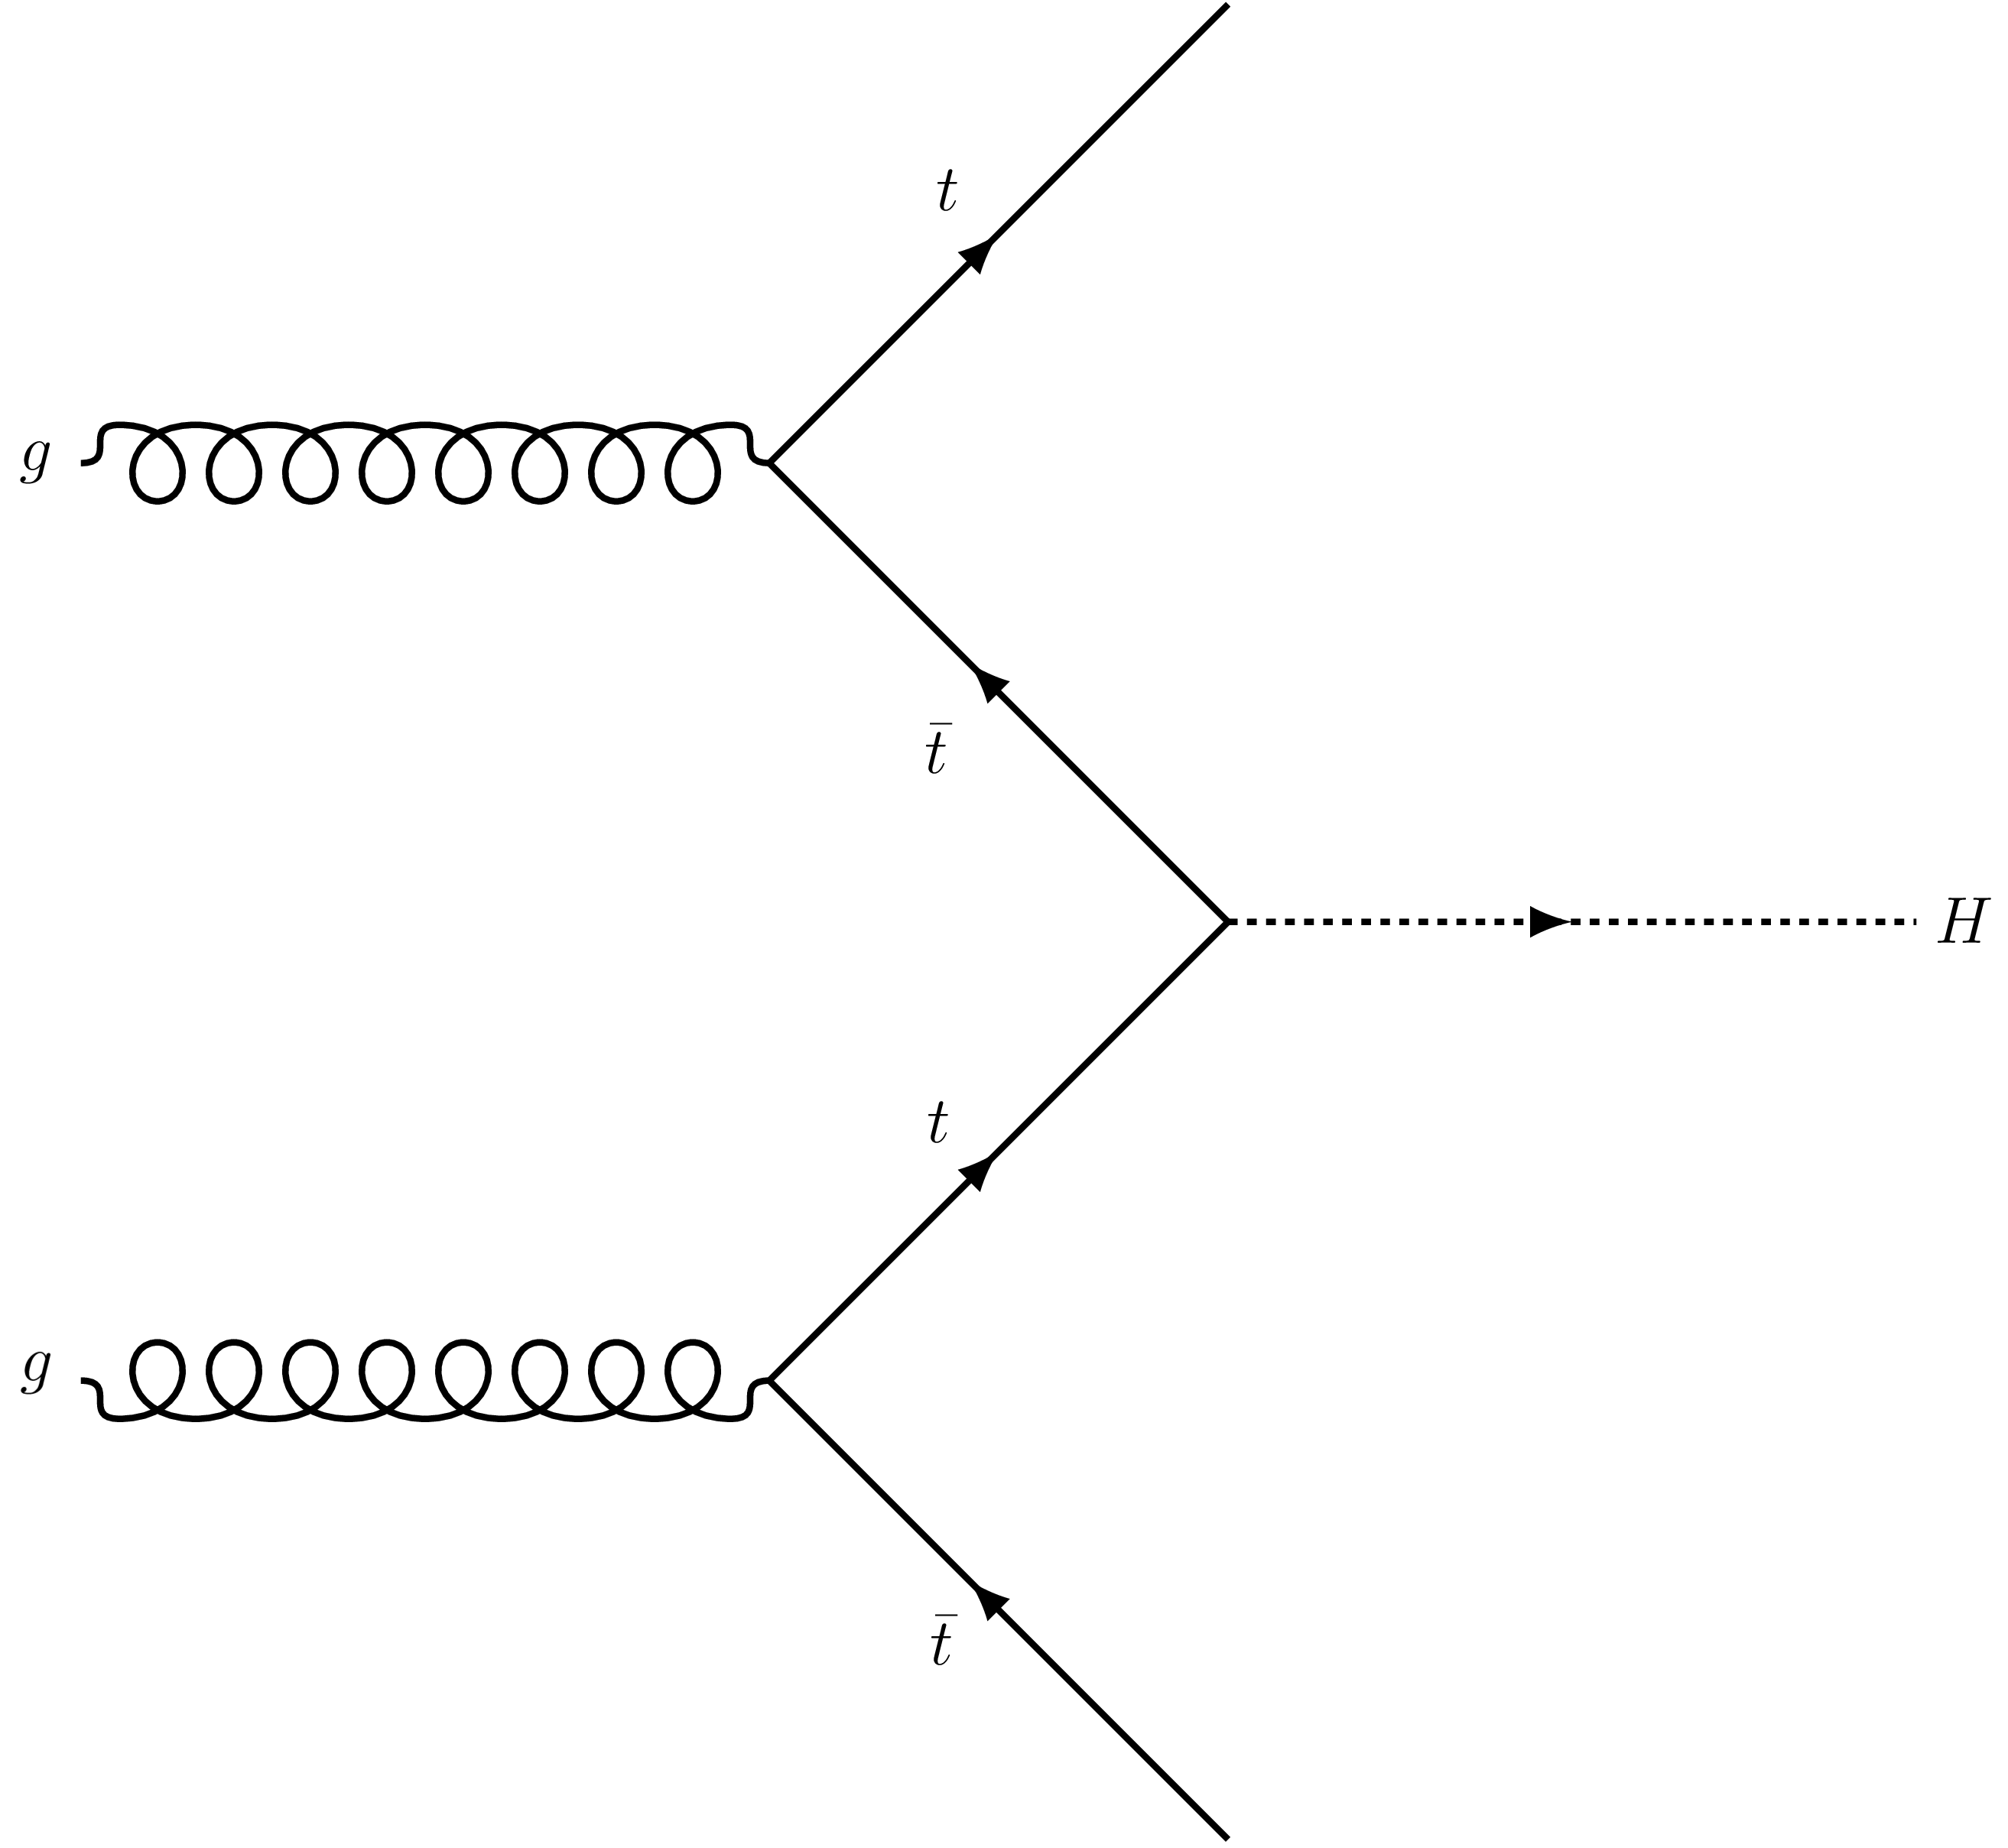
\includegraphics[width=\textwidth]{feynman_diagrams/ttH.png}
        \caption{\ttH}
    \end{subfigure}
    \hfill
    \begin{subfigure}[b]{0.45\textwidth}
        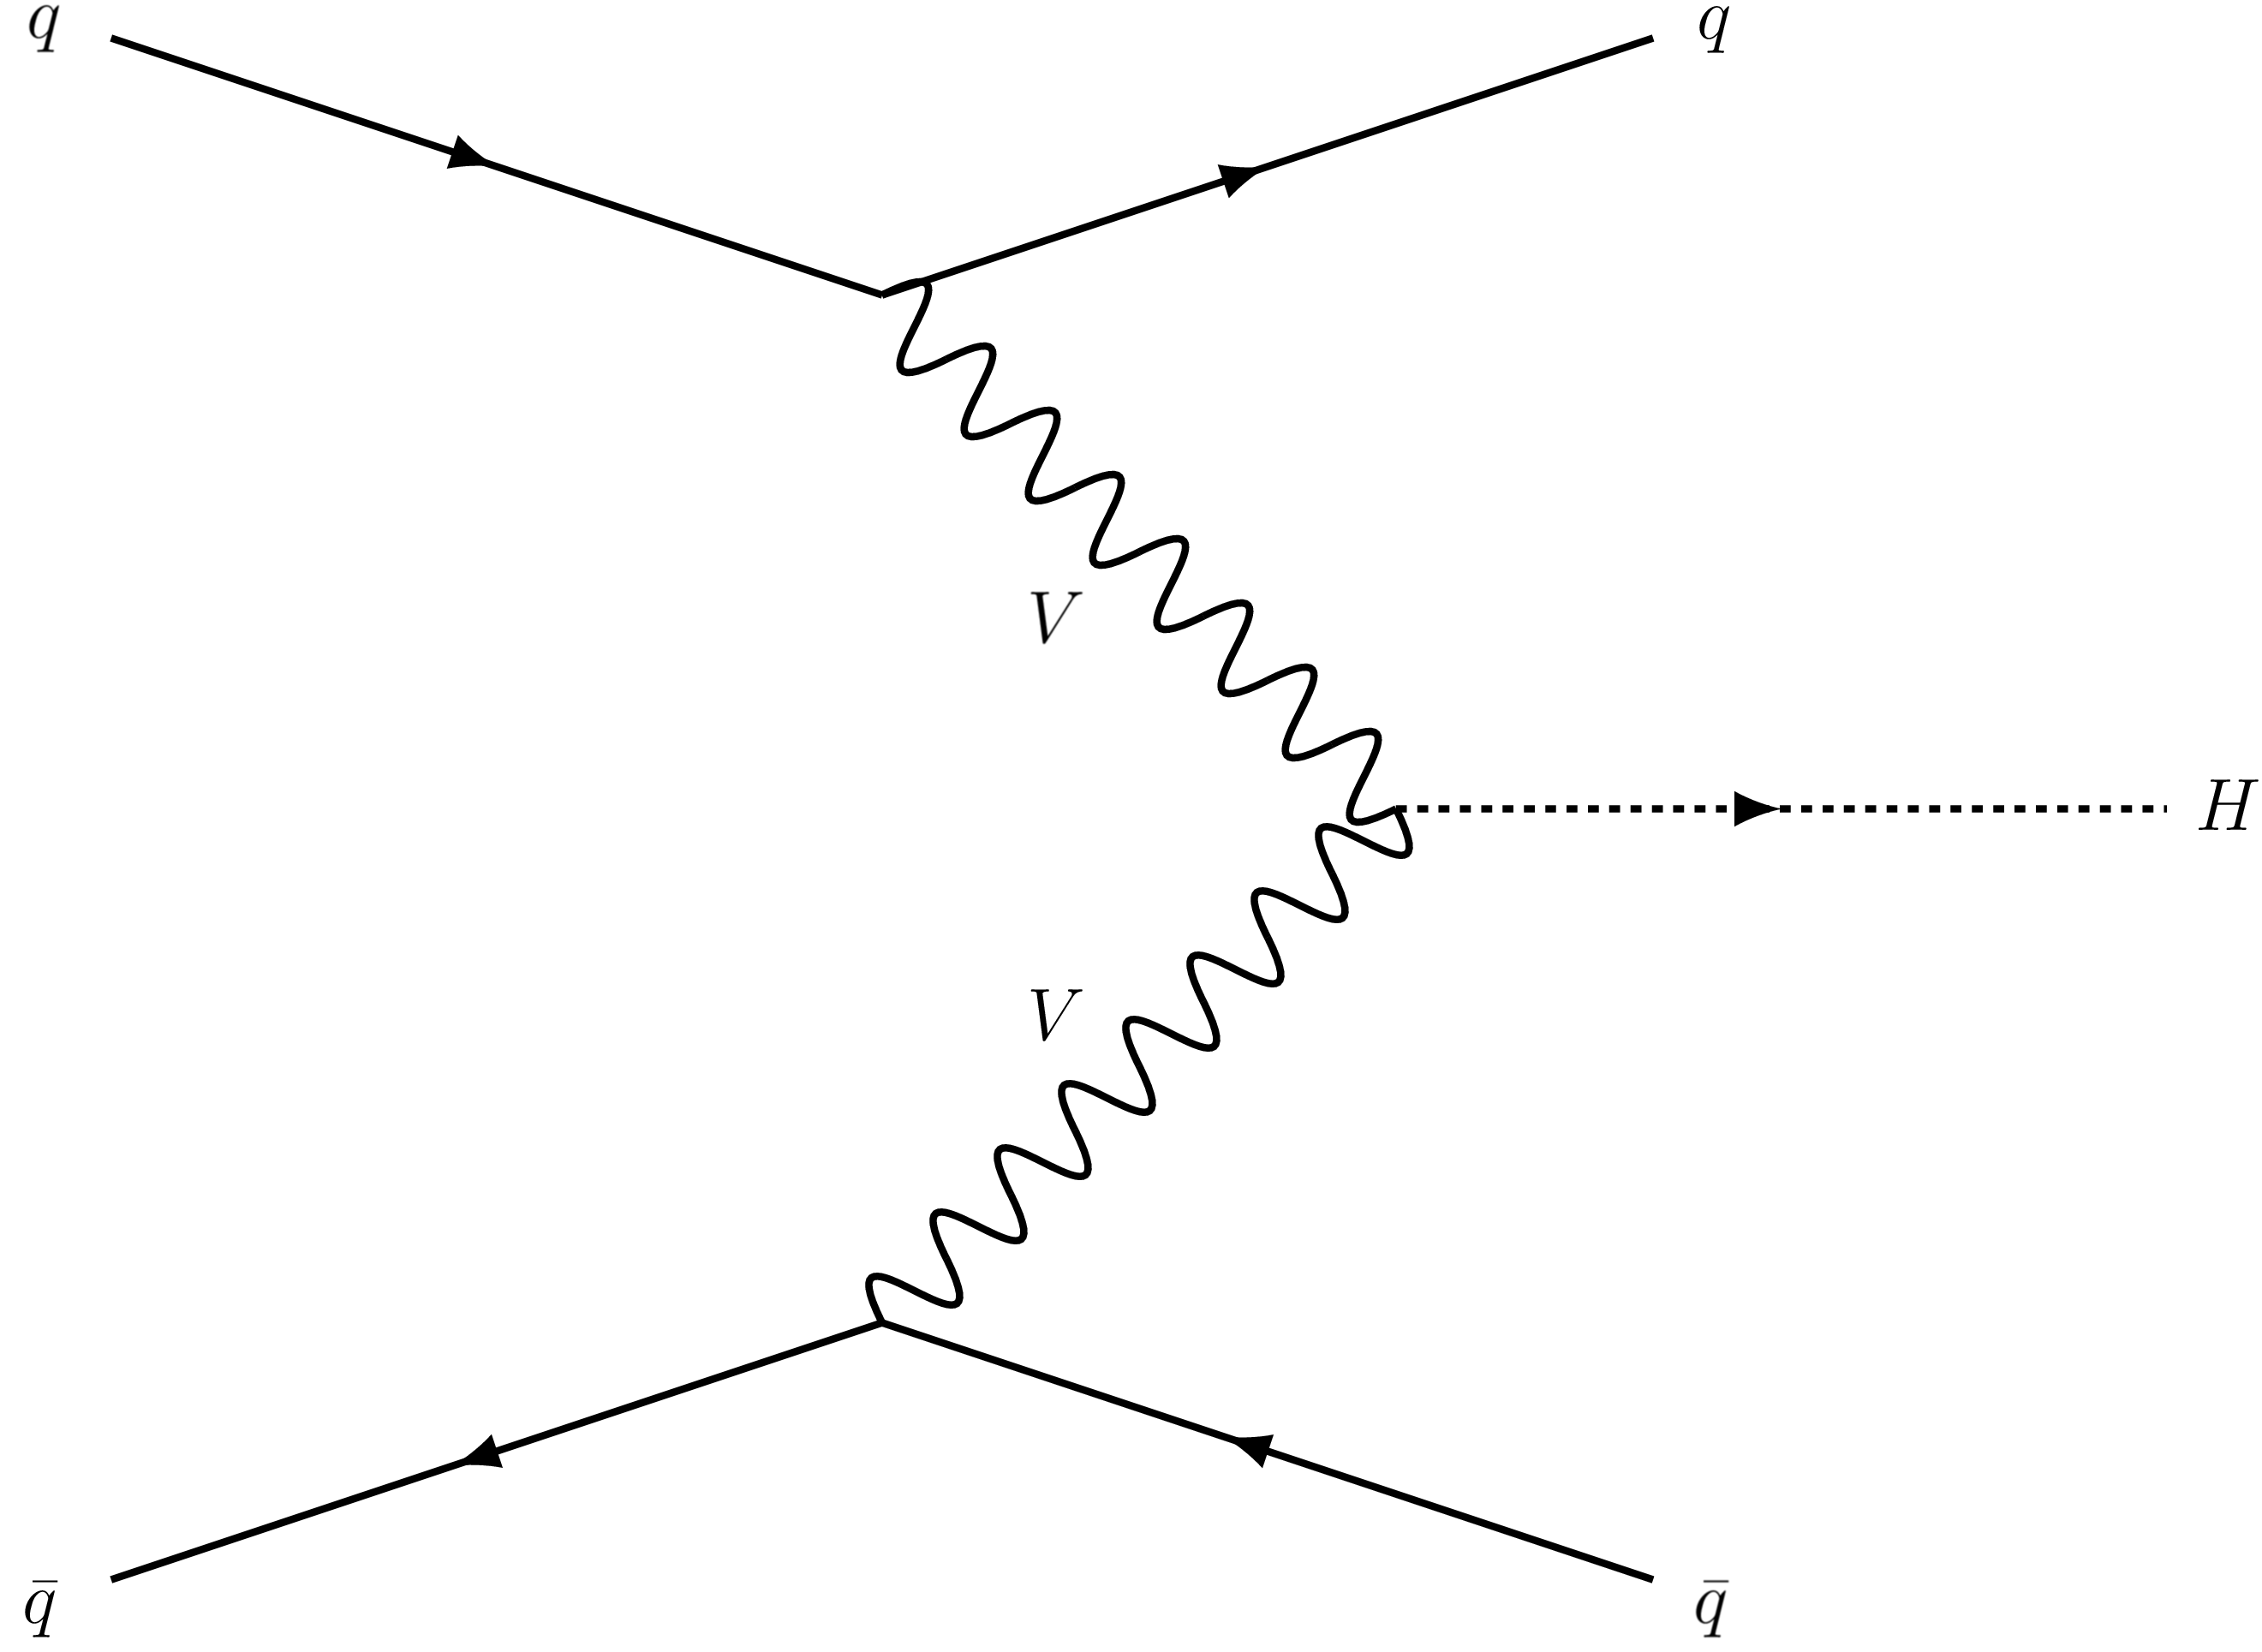
\includegraphics[width=\textwidth]{feynman_diagrams/VBF.png}
        \caption{VBF}
    \end{subfigure}
% blank line to start new row
    \begin{subfigure}[b]{0.45\textwidth}
        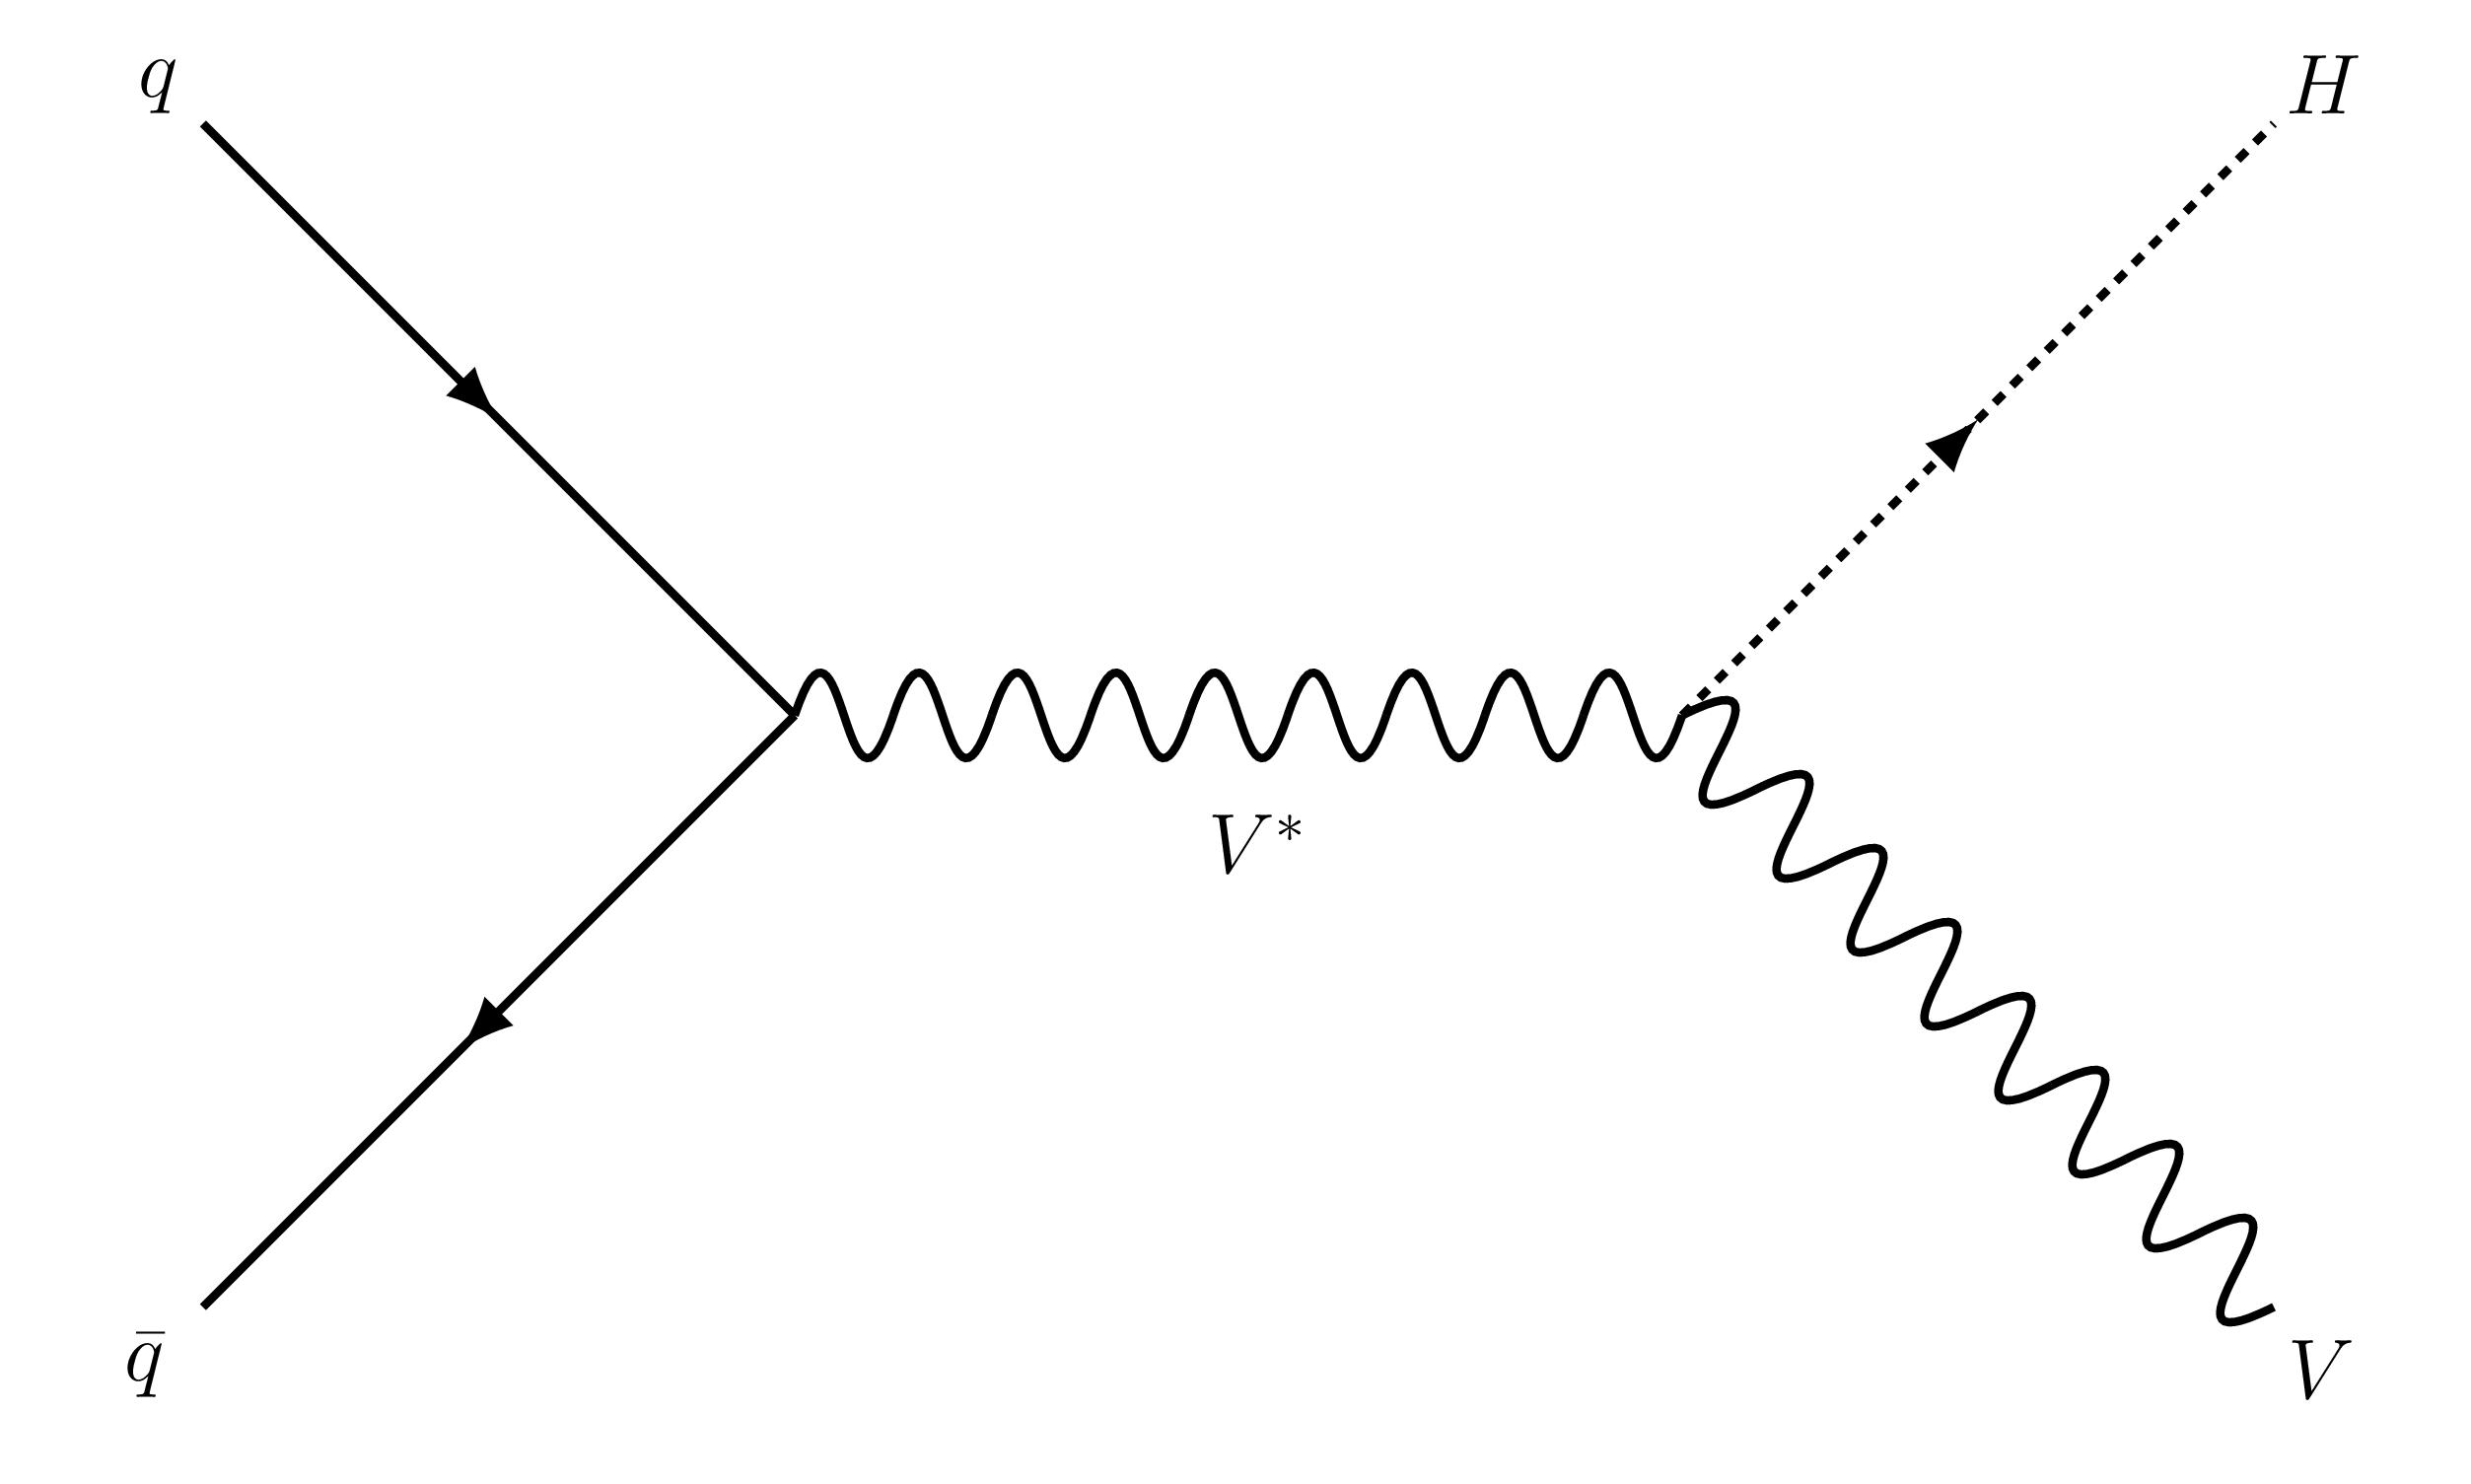
\includegraphics[width=\textwidth]{feynman_diagrams/VH.png}
        \caption{\VH}
    \end{subfigure}
    \hfill
    \begin{subfigure}[b]{0.45\textwidth}
        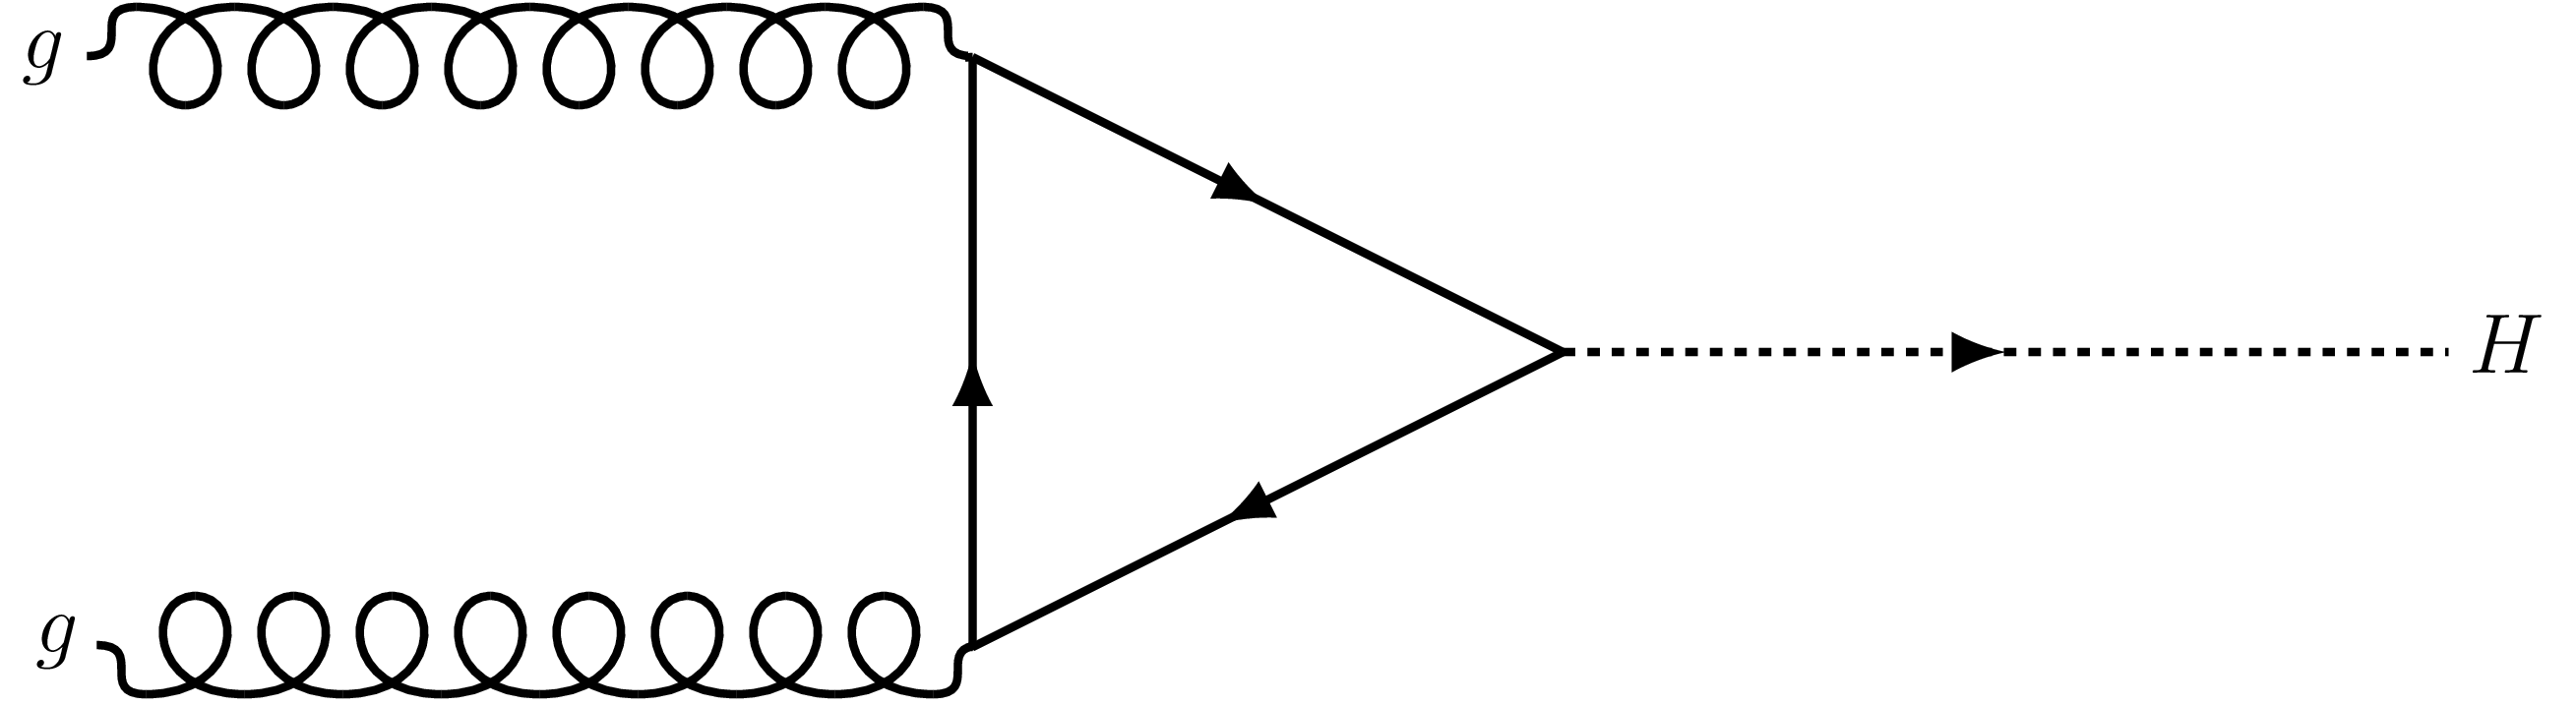
\includegraphics[width=\textwidth]{feynman_diagrams/ggF.png}
        \caption{\ggF}
    \end{subfigure}
\caption[The Feynman diagrams for the four main hadronic production modes of the Higgs boson]{The Feynman diagrams for the four main hadronic production modes of the Higgs boson.}
\label{fig:higgs_feynman_diagrams}
\end{figure}


%=========================================================


\section{Categorisation of the non-VBF production modes}
\label{sec:htoinv_categorisation}


%=========================================================


\section{Data and simulation}
\label{sec:htoinv_data_sim}


%=========================================================


\subsection{Weights and corrections for simulated processes}
\label{subsec:htoinv_mc_corrections}

% Pulled directly from AN. Tidy up
In order for simulated events, particularly for background processes, to resemble LHC data as closely as possible, many corrections and weights are applied. These are discussed in more detail in the following sections [REF]. A final event weight $w_{\mathrm{event}}$ is the product of the weights from all of the individual sources $i$ that provide a weight:

\begin{equation}
\label{eq:event_weight}
w_{\mathrm{event}} = \prod_i w_i
\end{equation}

When representing these events in histograms, the yield in a given bin $N_{\mathrm{corr.}}$ is the sum of these event weights:

\begin{equation}
\label{eq:bin_weight}
N_{\mathrm{corr.}} = \sum_j^{N_{\mathrm{MC}}} w_{\mathrm{event} \ j}
\end{equation}

where $N_{\mathrm{MC}}$ is the number of unweighted simulated events in the bin. The statistical uncertainty ascribed to the yield in a bin is given as

\begin{equation}
\Delta N_{\mathrm{corr.}} = \pm \frac{ N_{\mathrm{corr.}} }{ \sqrt{N_{\mathrm{MC}}} }
\label{eq:uncertainty_mc_ours}
\end{equation}

The statistical uncertainty for the number of events in data is simply the Poissonian error

\begin{equation}
\Delta N_{\mathrm{data}} = \pm \frac{ N_{\mathrm{data}} }{ \sqrt{N_{\mathrm{data}}} }
\label{eq:uncertainty_data}
\end{equation}

The standard prescription for error propagation is to approximate the uncertainty as the square root of the sum of the weights squared~\cite{bevington2003data}:

\begin{equation}
\Delta N_{\mathrm{corr.}} = \pm \left( \sum_j^{N_{\mathrm{MC}}} w_{\mathrm{event} \ j}^2 \right) ^{1/2}
\label{eq:uncertainty_mc_normal}
\end{equation}

Our reasoning for using Eq.~\ref{eq:uncertainty_mc_ours} instead of Eq.~\ref{eq:uncertainty_mc_normal} is that the error should be determined purely from the integer number of events we select ($k$ in a Poisson statistical treatment), regardless of whether they are weighted or not. This often reduces the uncertainty for MC compared to Eq.~\ref{eq:uncertainty_mc_normal} since many more events are generated to predict a given equivalent luminosity. Further justification is that it is a good approximation in our assumed regime where we expect a large number of events from our MC samples before any cuts are applied (say $N$), and a large enough number of events after the cuts such that we do not encounter the low-$k$ or low-$N$ limits of Poissonian error propagation.


%=========================================================


\subsubsection{Cross section reweighting}
\label{subsubsec:xs_weighting}

Since an arbitrary number of events can be generated for simulation, and a larger number of events gives higher statistical power, events in these datasets need to be reweighted to normalise their contribution to a given region or category. To first order, the weight applied is

\begin{equation}
w_{\sigma} = \frac{ \sigma \intlumi }{ N \varepsilon }
\end{equation}

where $\sigma$ is the cross section of the process at the order it was generated (e.g., on DAS/XSDB for public datasets), \intlumi is the integrated luminosity of the LHC data it is being compared to, $N$ is the number of events in the dataset before any skimming (or the sum of the generator weights), and $\varepsilon$ is the filter efficiency (assumed to be unity for all datasets since no generator-level cuts are applied). If a dataset is generated at leading order, higher order corrections are usually applied on an event-by-event basis that changes the shapes of distributions (see [SEC ON NLO CORRECTIONS]). In some circumstances, ``flat" k-factors can be applied to a dataset that only alters the normalisation (i.e., its cross section).


%=========================================================


\subsubsection{Pileup}
\label{subsubsec:pu_reweighting}

Pileup interactions at the LHC are frequent (see Chpt.~\ref{subsec:pileup}) and must be modelled appropriately in simulation. Simulated samples are generated with a certain distribution of the number of pileup interactions which usually does not match the data recorded by CMS. This is due to changing conditions in the beam over a period of data taking. In order to make them comparable, the simulated events are reweighted; in this context it is known as \emph{pileup reweighting}. \texttt{ROOT} files containing histograms of the number of pileup interactions from short runs in the LHC are available centrally and are used as the reference for which to reweight the simulated events.

In the trees of the simulated samples, the branch \texttt{Pileup\_nTrueInt} is the mean of the Poisson distribution from which random numbers are drawn. In each simulated event, these random numbers (all from the same distribution) are used to set the number of in-time pileup interactions as well as the number of the interactions in each neighbouring bunch crossing to simulate the out-of-time pileup. In data, the same branch gives the average number of pileup interactions for a colliding bunch pair in a lumi section. The distribution of \texttt{Pileup\_nTrueInt} in the data is derived from the measured instantaneous luminosity for each colliding bunch pair in each lumi section and the cross section of the total inelastic pp interaction.

The nominal pileup weight, as well as the up and down systematic variations, for each simulated event are derived in nanoAOD-tools. %(\url{https://github.com/cms-nanoAOD/nanoAOD-tools/blob/048a828e1d7f5ac3346e2f5e7eafba2570e84bc4/python/postprocessing/modules/common/puWeightProducer.py}). % add a note about the min bias cross sections from the samples used to derive the data distributions for each year?


%=========================================================


\subsubsection{Veto and selection weights}
\label{subsubsec:veto_sel_weights}

In an analysis, events are often rejected by placing kinematic or object-based requirements. This type of selection strictly removes an event from the analysis if the requirement is not met. While kinematic requirements are either fulfilled or not, a different approach can be used when selecting the number of objects, i.e., when defining control regions. For a set of objects, the selection weight at event level is defined as

\begin{equation}
    w_{\mathrm{sel.}} = \prod_i^{N_\mathrm{objects}} \epsilon_i
    \label{eq:event_selection_weight}
\end{equation}

where $\epsilon_i$ is the efficiency/scale factor applied to object $i$. Only reconstructed (``reco'' level) objects that have been matched to a generator level object are considered. For leptons (\Pe, \Pmu, \Ptau) and photons, these scale factors are typically from the reconstruction efficiency, identification efficiency, and \pt- or $\eta$-dependent energy corrections. In the case of \Pqb-tagged jets, it is the data-MC scale factor at the given working point of the algorithm used to identify them. These weights are calculated individually for each type of object in an event, and individually for each source since they also introduce systematic variations that cannot be trivially aggregated. A veto weight is defined as

\begin{equation}
    w_{\mathrm{veto}} = \prod_i^{N_\mathrm{objects}} 1 - \epsilon_i
    \label{eq:event_veto_weight}
\end{equation}

The uncertainties/systematic variations follow the same prescription. With these quantities defined, an event that meets the object criteria is given the selection weight, otherwise it is given the veto weight. For example, if an event with one muon that meets the criteria for the \singleMuCr region will enter that region with its selection weight. That same event can also enter the signal region or one of the sidebands (depending on the event kinematics) with the veto weights. This ``migration'' of events, where they are able to contribute to more than one region, and the fact that weights are applied instead of event rejection, provides a noticeable decrease to the \acrlong{mc} statistical uncertainty in a given bin of a given distribution.

One thing must be noted about the migration of events, since we have many different regions of phase space in the analysis. The signal region and the sidebands have orthogonal kinematic requirements, so an event cannot enter the signal region \emph{and} one of the sidebands. The same is true amongst the control regions, i.e., an event cannot enter more than one of them due to the designed orthogonality. An event \emph{is} able to enter the signal region or a sideband with $w_{\mathrm{veto}}$, and also one of the control regions with $w_{\mathrm{sel.}}$. Since events in data are not weighted, they may only enter a single region.


%=========================================================


\section{Triggers}
\label{sec:htoinv_triggers}

\section{Background estimation}
\label{sec:htoinv_background_est}

\subsection{Control regions}
\label{subsec:htoinv_crs}

\subsection{Sidebands to the signal region}
\label{subsec:htoinv_sidebands}

\subsection{Background estimation methods}
\label{subsec:htoinv_background_methods}
